\section{Efficiency}

\subsection{Function Relocation}
The use of relocation at the function level in our instrumentation strategy stems from the fact
that we are performing the instrumentation statically on a platform that uses a
variable-length instruction set and it may not be always possible to instrument
an arbitrary point in the executable due to the lack of enough space for jump instruction to the instrumented code. 
A typical strategy used by static
instrumentation tools on platforms with fixed-length instruction sets is to
replace a single fixed-length instruction at the instrumentation point with a
branch instruction that will transfer control to the instrumentation code. This is fairly straightforward because by the
definition of a fixed-length instruction set, the instruction being replaced and
the replacing jump have the same length. Performing static instrumentation
in a variable-length instruction set does not afford us this luxury. In x86 platforms, a
jump instruction that uses a 32-bit offset requires 5 bytes, whereas for some of
the instrumentation points that interest us, there may not be enough space due
to several reasons including the size of basic block or whether it falls in between the target
of another jump/branch instruction in the original text of the executable.

This leaves two options for how to transfer control to the instrumentation code.
We must either use a technique entirely distinct from the idea of using a single
unconditional branch to execute the control transfer such as multiple shorter
jumps or software interrupts and traps, or we must somehow alter the application code so
that it can accommodate a single large control instruction that is larger than
the original amount of space available at the instrumentation point. A separate
technique for transferring control flow could be to use a series of branches,
where the instruction in the instrumentation point is a small branch that
transfers control to a larger intermediate branch. We do not consider this
method any further because the smallest unconditional branch instruction is 2
bytes in length, making it ultimately a half measure since there are
instrumentation points with only a single byte available to them. Besides, this technique would
require additional space to be inserted in the text section in the close proximity of
the instrumentation points. Another option
to consider is the method proposed by the BIRD project \ref{nanda2006bird}, which
proposes the use of the single-byte \begin{it}INT3\end{it} instruction, a single-byte
interrupt intended to be used by debuggers to set breakpoints. When a larger
branch won't fit within the specified area. This instruction is functionally
perfect for static instrumentation because it consumes only a single byte and
allows us to transfer control to an arbitrary location by registering an
exception handler with the system. We performed a cursory study on this scheme
from an efficiency standpoint to determine whether it was worth further
investigation. On a small benchmark set, our implementation of using
\begin{it}INT3\end{it} only when 5-byte unconditional branches do not fit at
the instrumentation point introduces slowdown of no less than 100-fold for
even a simple task of counting the number of executions of each basic block in the code. As one might
expect, this mechanism is unsuitable for efficient instrumentation since the
very heavyweight system call conventions are being invoked fairly often.

In PIX, we use the reorganization of the code at the function level so that
there is enough space at every instrumentation point to accommodate a 5-byte
branch. Specifically, the steps in whole function relocation includes function displacement, linking function entry points,
branch conversion and instruction padding.  \textbf{(COMMENT: What about the targets of branches in to the middle?)}
Figure \ref{Figure:Relocation} presents the flow of information on this process with a simple example function in the original text section
of an executable.

\begin{figure}[ht]
\centering
\caption[Optional caption for list of figures]
{The steps taken in order to prepare a function for instrumentation which collects
the memory addresses of an application.}
\subfigure[The two-segment structure of an unmodified ELF file.]{
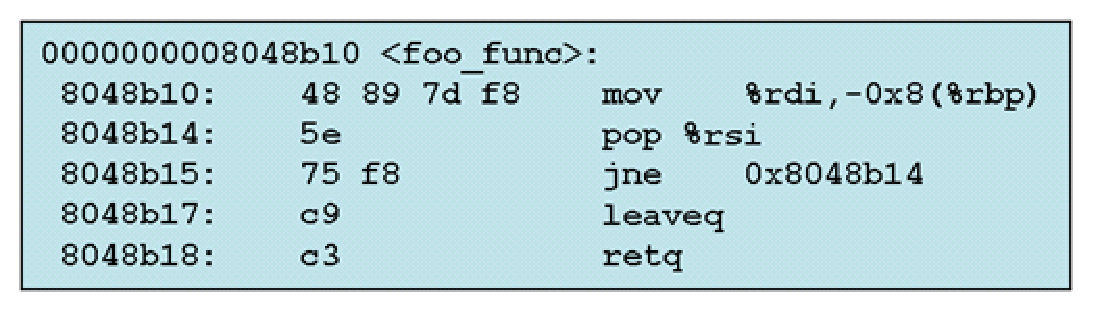
\includegraphics[scale=0.38]{funcp1.eps}
\label{Figure:funcp1}
}
\subfigure[The two-segment structure of an unmodified ELF file.]{
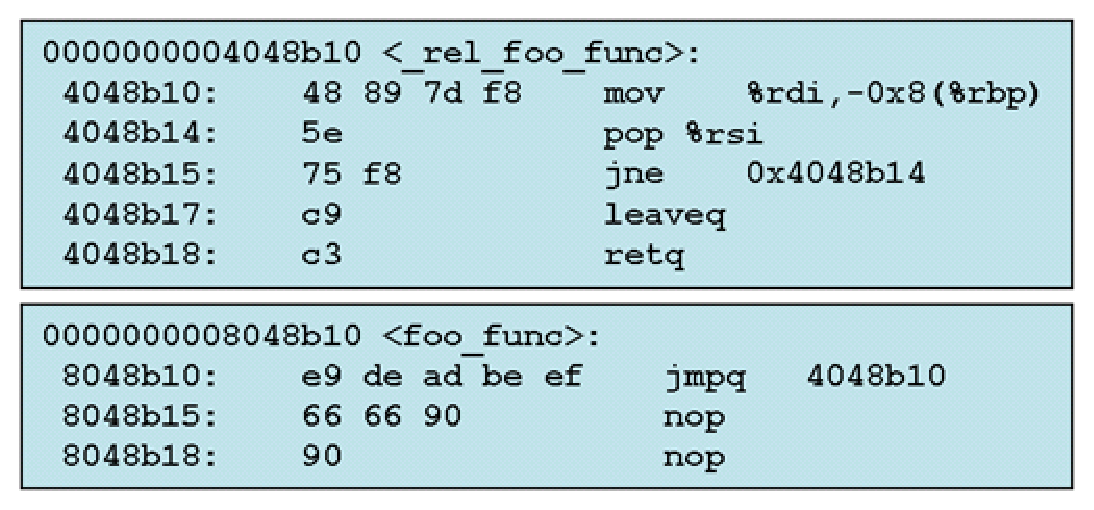
\includegraphics[scale=0.38]{funcp2.eps}
\label{Figure:funcp2}
}
\subfigure[The two-segment structure of an unmodified ELF file.]{
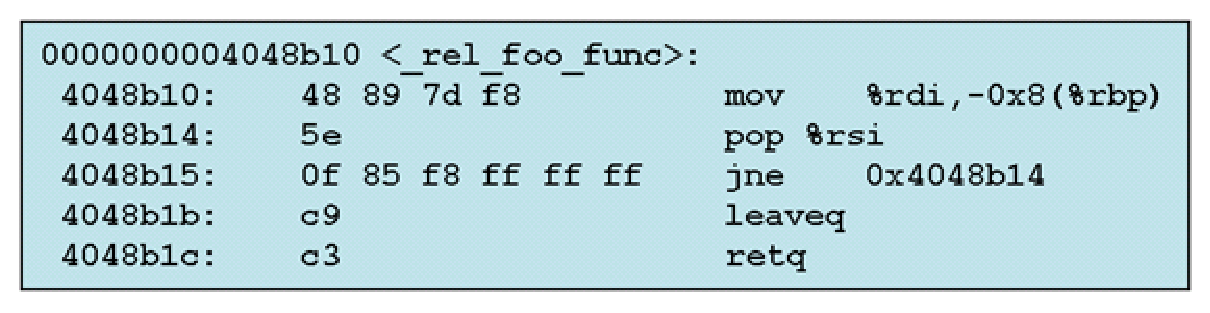
\includegraphics[scale=0.34]{funcp3.eps}
\label{Figure:funcp3}
}
\subfigure[The two-segment structure of an unmodified ELF file.]{
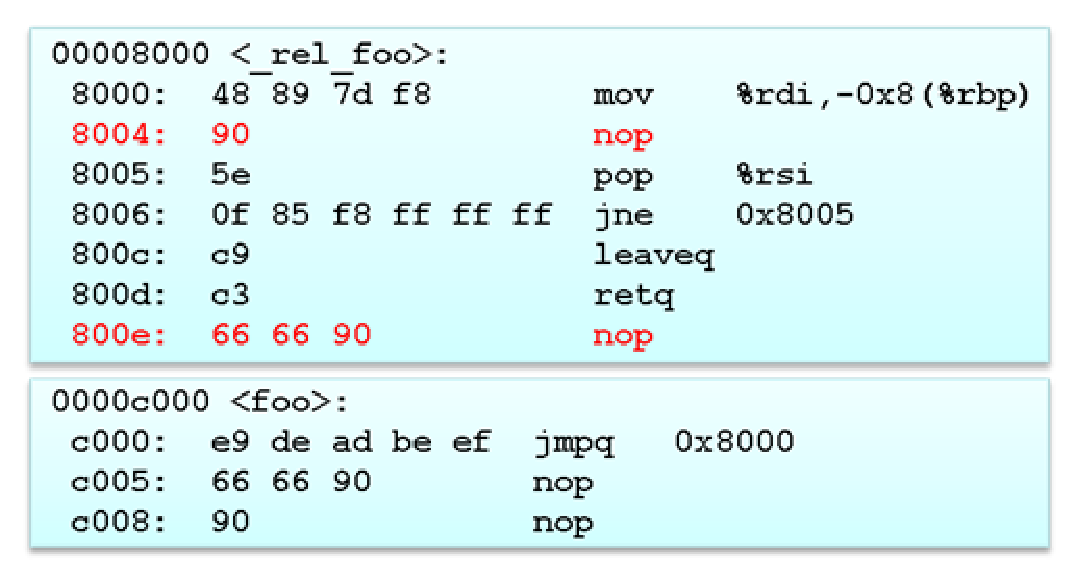
\includegraphics[scale=0.34]{funcp4.eps}
\label{Figure:funcp4}
}
\subfigure[The two-segment structure of an unmodified ELF file.]{
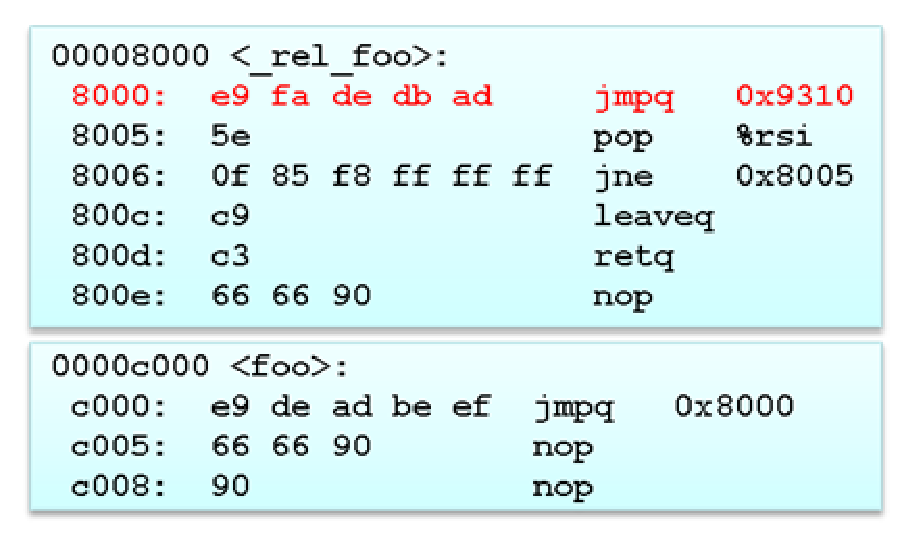
\includegraphics[scale=0.34]{funcp5.eps}
\label{Figure:funcp5}
}
\label{Figure:Relocation}
\end{figure}


\textit{Function Displacement} relocates the contents of the entire function to an area of the text section allocated
for the instrumentation tool. Since functions are often packed tightly together, it is generally not possible to
expand the size of a function without disturbing the entry points of another function using the original location of a function. 
\textit{Linking Function Entries} places an unconditional branch at the former function entry point that transfers control
to the new relocated function entry point. Most references to the entry point of a function are in the form of function calls, which
routinely are indirect references (i.e. their value is computed or looked up at runtime) and are difficult to resolve
prior to runtime. \textit{Branch Conversion} converts each short conditional branch in the relocated function to the equivalent
5-byte branch instruction. Since the code is being reorganized in the next step which may strain the limits of
smaller 8-bit or 16-bit offsets, we convert all branches to use 32-bit offsets so that the targets of each branch
will still be reachable without having the need to further reorganize the code. Note that there is opportunity
here to reduce space by using the smallest branch offset size that accommodates the branch, but we chose to use a single 
mechanism to simplify the implementation and optimize the space usage in the future. \textit{Instruction Padding} pads
the instruction at each instrumentation point with \begin{it}nop\end{it} instructions so that a 5-byte branch can fit
 according to the needs of the instrumentation tool. 

There are several ways that whole function relocation may adversely affect 
the performance of the instrumented executable independent of the overhead
that will be imposed by the additional instrumentation code. Each function call
now has an extra control interruption associated with it since control must be passed first to the original function entry
point and then to the relocated function entry point. It is possible that using 32-bit offsets for every branch rather than
some smaller number of bits has an overhead associated with it. And since the code is being reorganized and expanded, 
we might destroy some positive alignment and size optimizations that the compiler might have made on the instructions in the
function. To quantify the impact of whole function relocation on the performance of applications, we conducted several experiments
where we generated executables in which only functions are relocated and no instrumentation code is inserted and compared 
their performance to the original executables. Thus, we examine the practical overhead seen by these techniques 
by taking these steps without instrumenting the code for a series of benchmarks. The results of these experiments are described 
in detail in Section SSSS but in the average the slowdown incurred by whole function relocation is XXXX in the average, which is
negligible.

\subsection{Disassembly Coverage}
Code and data can reside together in the text section of a program binary. This is done for a variety of reasons, including
the storage of branch target locations (eg for a jump table) or small data structures that provide convenient look-up
of certain data such as identifiers, descriptors, or other values.

Correctly determining
what parts of the text sections are code and what are data is important. Consider what can happen
if we mistakenly treat some data as code. We might choose to modify or relocate the apparent code
to serve our instrumentation purposes. Then when the data at this location is referenced, the
original program behavior may not be preserved: if we are lucky this will cause application failure
due to some unexpected change in control flow or some state condition that is checked by the program.
If we are unlucky the corruption might silently manifest itself by modifying the output of the
program. Alternatively consider what can happen if we mistakenly treat some code as data. We then will
not try to insert code into this area or we might perform some other type of analysis that should be reserved for
data alone. While this is almost certainly preferable to the situation where we treat data as code, it
is ideal to avoid both situations.

To this end, we use the program's symbol table to help us determine which parts of the text sections
are functions that are eligible to be subject for our code discovery algorithm. Our code discovery algorithm
consists of two phases; control-driven disassembly backed up by linear disassembly. In more detail, the algorithm
works as follows:

\begin{enumerate}
\item 
1. Control-driven disassembly: from a function's entry point, follow all understandable control paths. If a problem is encountered, fall back to
naive disassembly.
\item
2. Naive disassembly: from a function's entry point, disassemble each instruction in the order it appears in the
function. If a problem is encountered, give up.
\end{enumerate}


Problems that can be encountered are situations where an unknown opcode is encountered, where control jumps to the
middle of an instruction we've already disassembled, or if control leaves the boundaries of the function. In most
cases control-driven disassembly is sufficient to disassemble the entirety of a function, and in most cases control-driven
disassembly is a straightforward process because control either falls through to the following instruction 
or the location of a branch target is embedded entirely within the instruction itself. But there are also cases
where the an indirect branch is used, where the target resides either at a fixed address (possibly with some offset), the address that resides in a register,
or the address that is at a location given by a register. The latter two cases are very difficult to resolve
without runtime information because the computation of the target address can be arbitrarily complex and can span function
boundaries. Nevertheless, we perform a peephole examination of the previous instructions to the and can determine 
the address in simple cases.

Fortunately simple calculations are all that most compilers use to determine targets for jump tables, one of the more common
uses of an indirect branch. Often an offset is added to a fixed location to determine where the data comprising the branch target
resides. Therefore we treat such a fixed address as the first entry in a table whose entries are treated either as addresses or as offsets.
We then make an iterative pass over this table to determine the target for each arm of the jump table, stopping when we find a value in the
table that yields an address that is outside the scope of the function.

PUT EXAMPLE OF GNU COMPILER JUMP TABLE HERE

\subsection{Instrumentation Snippets}

In most instrumentation tools, the tasks accomplished by the instrumentation tool are accomplished by allowing the user
to transfer control from instrumentation points in the application to instrumentation functions provided by the user, typically
via a shared library or some other type of object code. Since these instrumentation functions are delivered via a shared library or other
object code, the instrumentation tool developer has the advantage of the use of a software devlepment toolchain and can
write the code in a language that compiles to object code. This delivery mechanism is, however, somewhat heavyweight. Each time
the instrumentation tool needs to accompish any task, the overhead of a function invokation must be born. In cases where
efficiency is important and where the instrumentation task is relatively small, it can be desirable to insert small sequences of assembly code
to perform a task rather than relying entirely on more heavyweight instrumentation functions.

Consider the example of an instrumentation point where we wish to update a counter that resides in memory, which could be of particular use for
basic block or instruction counting tools. In order to accompish this task with an instrumentation snippet, we transfer control to the
instrumentation point's trampoline which will save athe flags register, update the counter in memory (this does not even require a register), restore
the flags register, then transfer control back to the application. Using an instrumentation function, prior to performing
the task the trampoline must save the flags register, any registers used by the function, and perform stack protection in some cases. 
The larger costs associated with using an instrumentation occur because the instrumentation function requires at least 2 more control flow transfers
to enter and exit the function. Furthermore these control flow transfers generally use the call/return paradigm, which in addition to changing the
application's program counter will also store and retreive information about the function call site onto the stack. There will also be some overhead
associated with setting up a stack frame for the instrumentation function. The use of the instrumentation function is also likely to pollute the
instruction cache more than using an instrumentation snippet. For an instrumentation snippet the application code must contend with the trampoline code
only, whereas using an instrumentation function puts the function code into contention with the other two as well.

These factors show us that instrumentation functions tend to be a much more heaviweight solution, which is not appropriate for certain kinds of instrumentation
tasks. This technique can allow us to more efficiently gather asynchronous program information, which intuitively can be thought of as any information that could be dumped to
disk an processed offline. The authors of \cite{gao2005aliter} show that using lightweight instrumentation snippets to buffer information
which is later processed by more heavyweight instrumentation functions in batches can be an efficient yet entirely lossless way of processing asynchronous
program information. The avaialability of instrumentation snippets gives tool authors the flexibility to choose between these and instrumentation
functions depending on their efficiency and software engineering needs.


% move this to overview section
The stack requires protection from the instrumentation function because compilers will often optimize a leaf function
by not explicitly creating a stack frame for the local function data to operate in. This optimization is safe for the application because during its
normal execution a leaf function will never call another function and thus its errant stack contents can never be smashed. In the case of an instrumentation
tool that calls an instrumentation function from a leaf, this guarantee no longer holds. Thus we must protect the area above the stack when we call
an instrumentation function from a leaf function. During the disassembly of a function we note whether it is a leaf (ie whether it contains any call
instructions), and then during instrumentation we automatically protect the stack contents for any instrumentation function calls that are made by
incrementing the stack pointer by a large fixed amount, which has the effect of giving the leaf function a large stack frame while the instrumentation
function's stack frame uses the stack.



